\documentclass[tikz,border=2pt]{standalone}
\usepackage{amsmath}
\usepackage{pgfplots}
\pgfplotsset{compat=1.18}
\usetikzlibrary{arrows.meta}
\begin{document}
% U[0,1] values, n = 4: G(x) = x^3. For a type theta (here theta = 0.8) the rectangle
% theta*G(theta) splits into the surplus U(theta) = int_0^theta G(x) dx (below the curve)
% and the expected payment m(theta) = theta G(theta) - int_0^theta G(x) dx (above the curve).
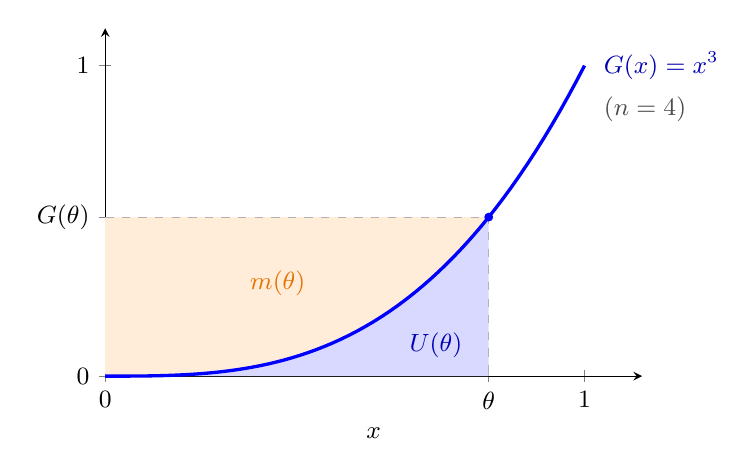
\begin{tikzpicture}[font=\small, >={Latex[length=2mm]}]
  \begin{axis}[
    axis lines=left, xmin=0, xmax=1.12, ymin=0, ymax=1.12,
    xtick={0,0.8,1}, ytick={0,0.512,1},
    xticklabels={$0$,$\theta$,$1$}, yticklabels={$0$,$G(\theta)$,$1$},
    xlabel={$x$},
    width=8.4cm, height=6cm, clip=false, samples=60]
    \addplot[fill=orange!15, draw=none, domain=0:0.8] {x^3} -- (axis cs:0.8,0.512) -- (axis cs:0,0.512) -- cycle;
    \addplot[fill=blue!15, draw=none, domain=0:0.8] {x^3} -- (axis cs:0.8,0) -- (axis cs:0,0) -- cycle;
    \addplot[gray!60, thin, dashed] coordinates {(0,0.512) (0.8,0.512) (0.8,0)};
    \addplot[blue, very thick, domain=0:1] {x^3};
    \fill[blue] (axis cs:0.8,0.512) circle (1.6pt);
    \node[orange!90!black] at (axis cs:0.36,0.3) {$m(\theta)$};
    \node[blue!70!black] at (axis cs:0.69,0.1) {$U(\theta)$};
    \node[blue!70!black, anchor=west] at (axis cs:1.02,1) {$G(x)=x^3$};
    \node[gray!60!black, anchor=west] at (axis cs:1.02,0.86) {($n=4$)};
  \end{axis}
\end{tikzpicture}
\end{document}
